%----------------------------------------------------------------------
%	DIRC TECHNOLOGY CHAPTER
%----------------------------------------------------------------------
\label{ch:components}
The validation of the key components of the DIRC for an EIC discussed in Chapter \ref{ch:eicdirc} is vital to show that the Geant4 simulation package produces results expected for the real detector. However, due to budget restraints it was not possible to build or otherwise procure a full scale prototype of the envisioned EIC DIRC discussed in Chapter \ref{ch:eicdirc} (e.g. $2\times2\unit{mm}^2$ pixel MCP-PMTs are not currently available commercially). Instead a series of test bench measurements have been made to validate simulated performance of the new 3-layer lens design, study the radiation hardness of the NLaK33 material, and evaluate the performance of MCP-PMTs in high magnetic field environments.

%----------------------------------------------------------------------
%	3-LAYER LENS OPTICS SECTION
%----------------------------------------------------------------------
\section{Optical Properties of 3-Layer Lens}
\begin{figure}[ht]
	\centering
	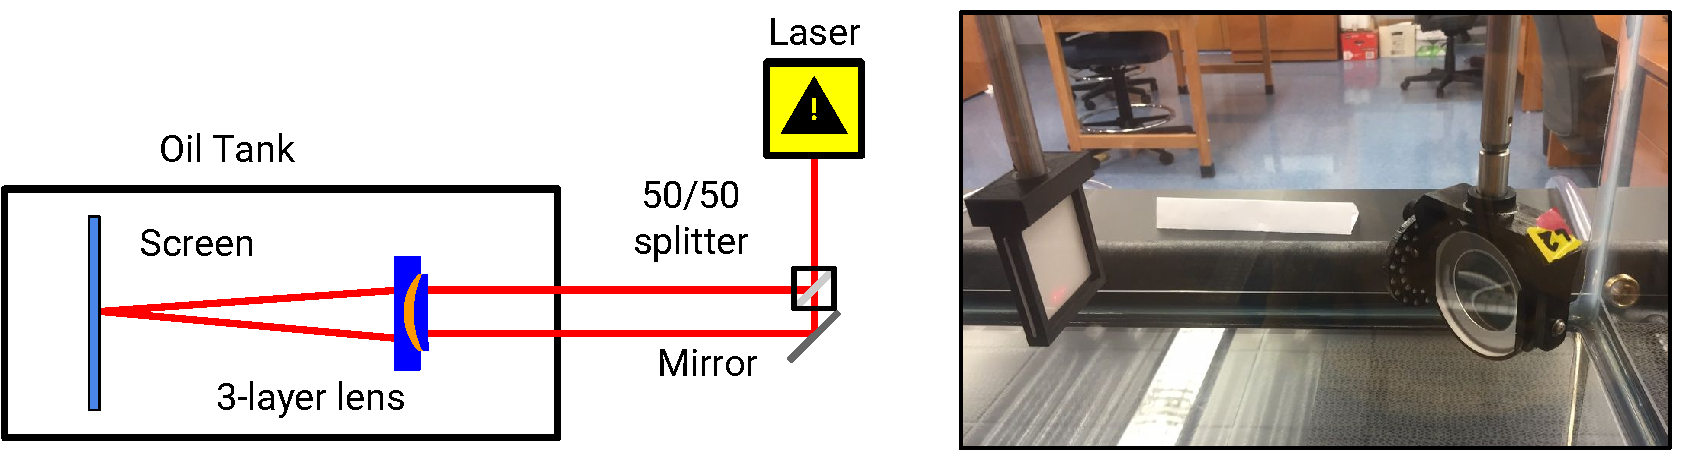
\includegraphics[width=\textwidth]{lens_setup_schematic.pdf}
	\caption{Schematic drawing of the setup built at Old Dominion University for testing the optical properties of the 3-layer lens design (left), and a closeup view of the lens and screen inside the actual setup (right).}
	\label{fig:ODU_setup}
\end{figure}

\begin{figure}[ht]
	\centering
	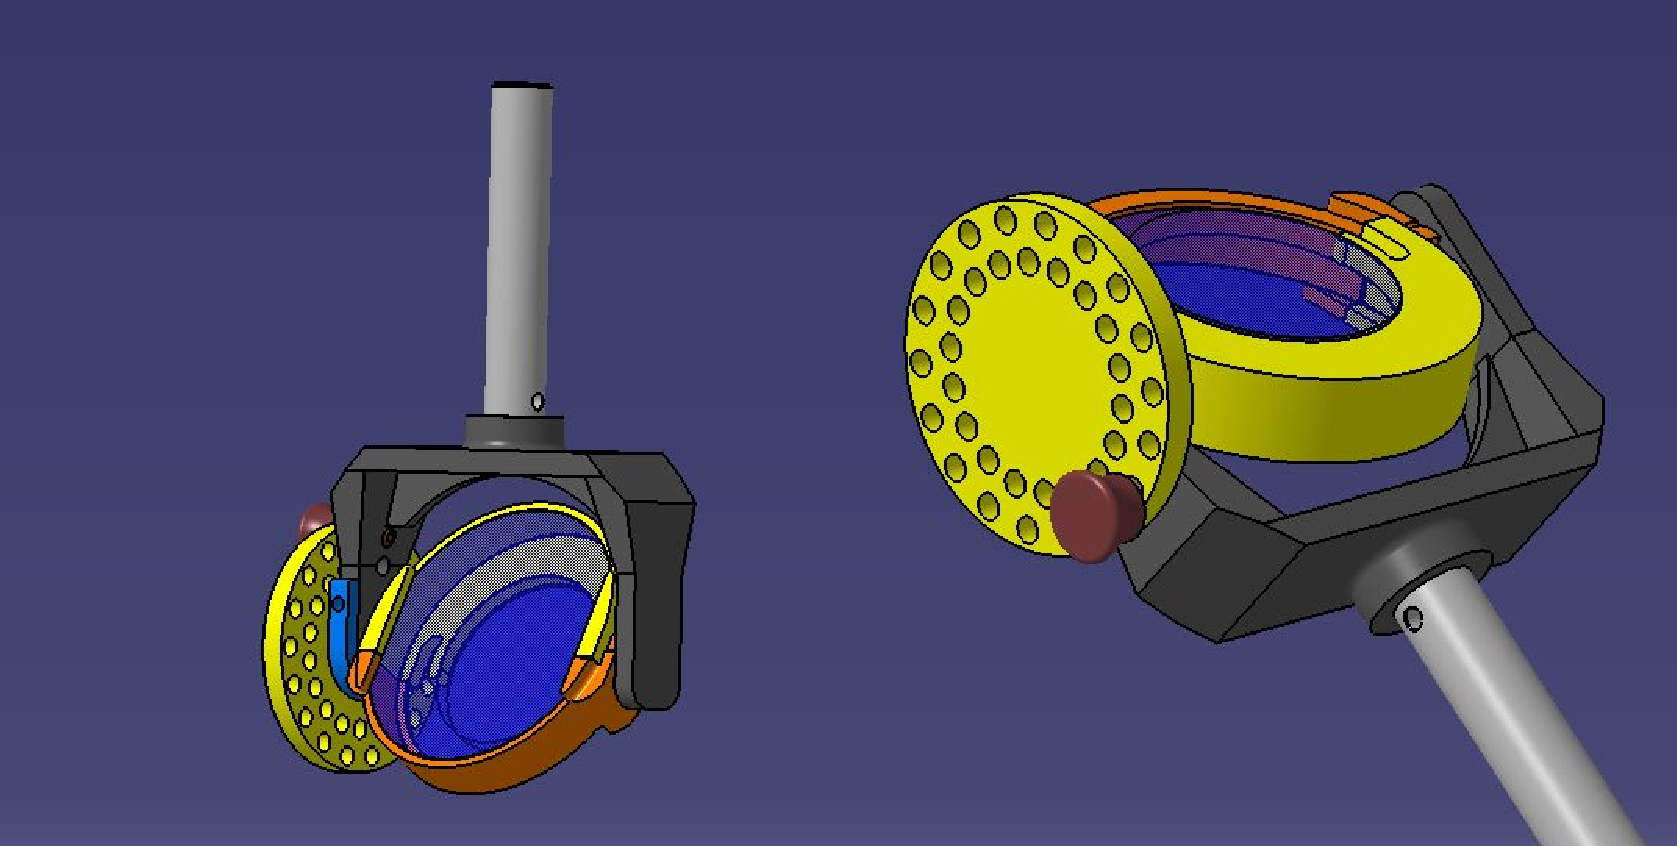
\includegraphics[width=\textwidth]{lens_holder.pdf}
	\caption{CAD drawing of 3-layer lens holder which lets the lens rotate in two planes, allowing the full 3D focal plane to be mapped.}
	\label{fig:lens_holder}
\end{figure}

\begin{figure}[ht]
	\centering
	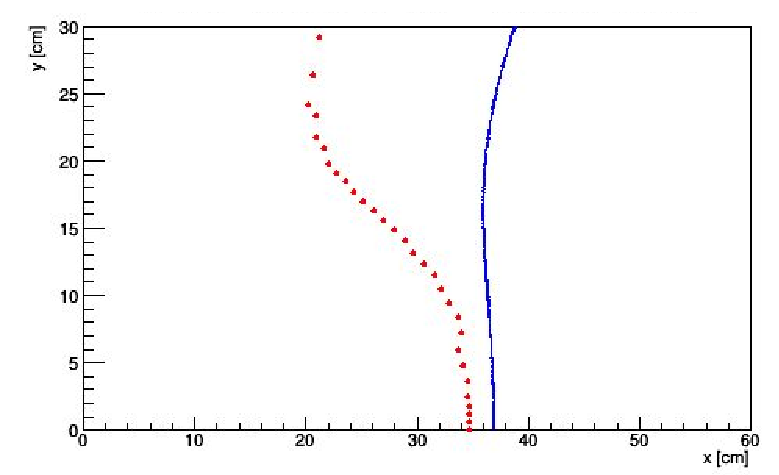
\includegraphics[width=\textwidth]{focalplane_initial.pdf}
	\caption{Initial measurement of the 3-layer lens focal plane using the upgraded green laser (red dots) compared to simulation (blue line).}
	\label{fig:focalplane_initial}
\end{figure}

\begin{figure}[ht]
	\centering
	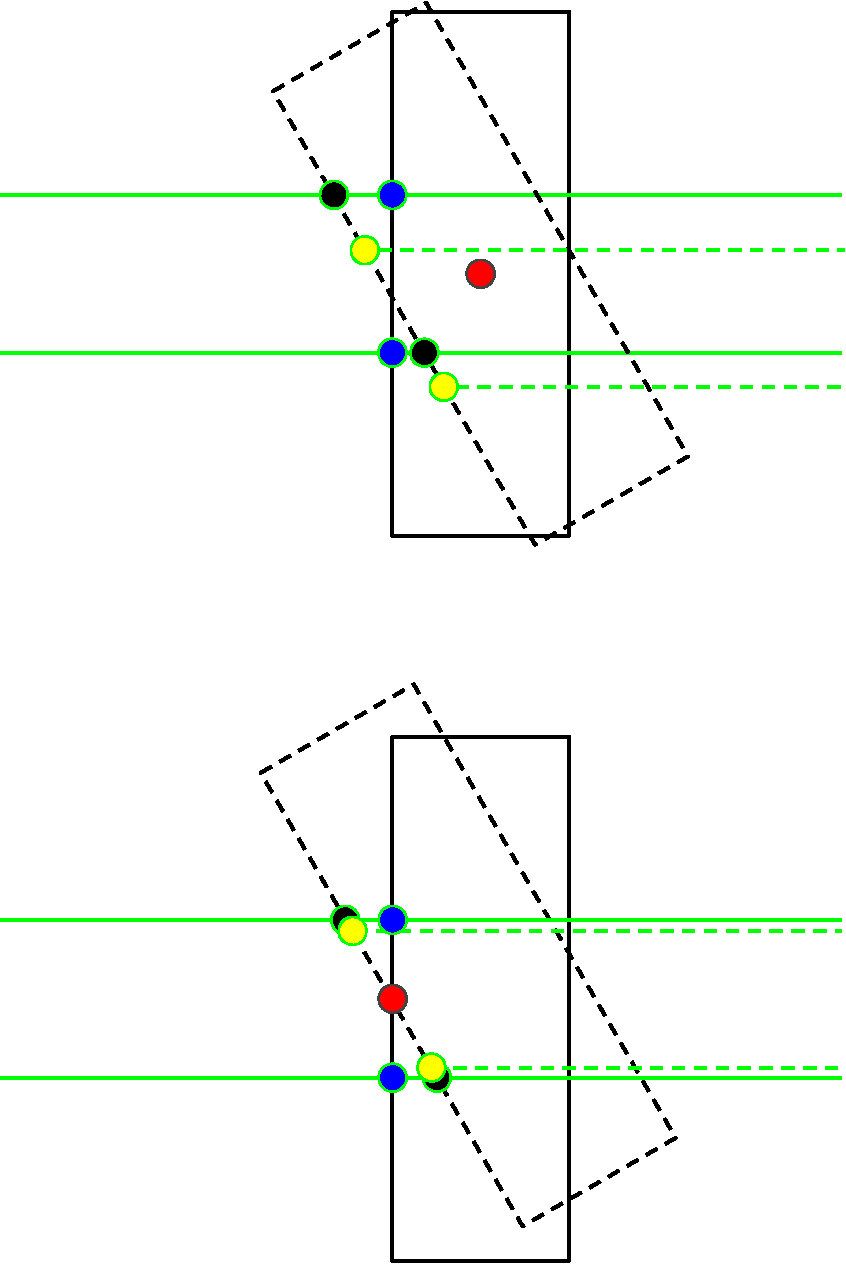
\includegraphics[width=0.43\textwidth]{lens_rotation_point.pdf}
	\caption{Schematic of the discrepancy between beam positions in data (black) and simulation (yellow) in relation to the original beam positions (blue) for a given rotation point (red) at the center (top) of the lens, or at the edge (bottom) of the lens. }
	\label{fig:lens_rotation_point}
\end{figure}

\begin{figure}[ht]
	\centering
	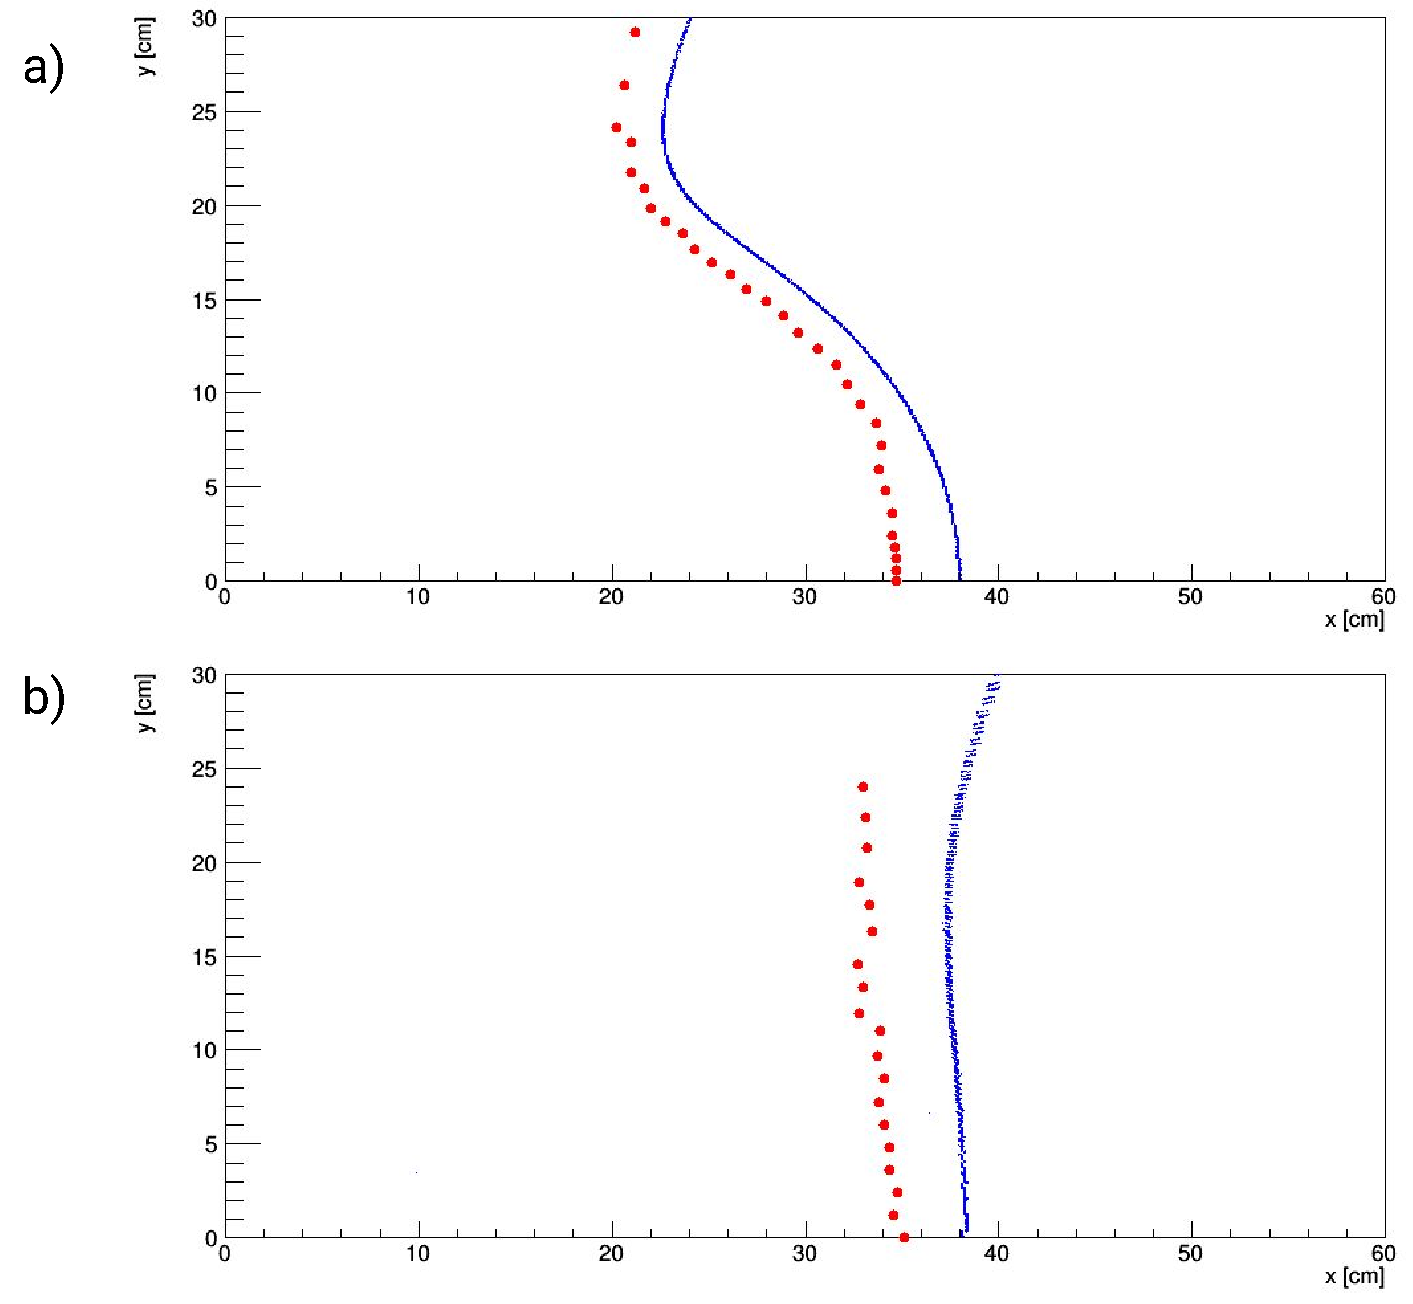
\includegraphics[width=\textwidth]{focalplane_corrections.pdf}
	\caption{Initial measurement of the 3-layer lens focal plane compared to a rotation corrected simulation (a), and a second measurement with a tighter (2 mm) beam configuration and a modified lens holder (b).}
	\label{fig:focalplane_corrections}
\end{figure}

To measure the shape of the focal plane a setup was designed and built at Old Dominion University, shown in Figure \ref{fig:ODU_setup}, in which a laser shines through a 50/50 beam splitter and a mirror to make two beams that are parallel to within 0.5 degrees across roughly 10 meters. The beams then pass through a $30\times40\times60\unit{cm}^3$ glass container filled with mineral oil with a refractive index similar to that of fused silica to simulate the behavior of light passing from bar to lens to expansion volume. The beams are focused through the 3-layer lens, being held in a specially designed holder that allows the lens to be rotated in two planes (Figure \ref{fig:lens_holder}). Finally the beams are focused onto a plastic screen inside the tank and intersection of the two beams determines the focal length.

Measurements were initially taken with a 632 nm red helium-neon laser, but the beam spot was too large and very distorted. A 530 nm wavelength green laser with a 1 mm beam spot was then purchased to replace the red laser. Initial results with a 5 mm beam separation are shown in Figure \ref{fig:focalplane_initial}. Obviously there is a large discrepancy in both position and shape of the measured and simulated focal plane. This was rectified by discovering that in the simulation it was assumed that the two beams were entering the lens at fixed points on the lens' face regardless of lens rotation, where as in the experiment the rotation of the lens about it's center causes the beams to shift with respect to the lens face. When rotating at the edge of the lens closest to the laser rather than through the center this difference is negligible, as illustrated in Figure \ref{fig:lens_rotation_point}.

A correction was implemented in the Geant4 simulation to account for the shift of the beam spot during rotation, the results of which can be seen in Figure \ref{fig:focalplane_corrections}a. The beams have since been brought to a 2 mm separation to reduce effects of aberration and a second lens holder was 3D printed to allow for rotation about the edge of the lens. A new round of data was taken and results are shown in Figure \ref{fig:focalplane_corrections}b. This change vastly improved the results of both the simulation from the first measurement and the results of the second, showing that the simulation indeed reproduces very nicely the shape of the focal plane, although the position is still roughly 3 cm too long. This could be explained by reducing the radius of the second layer of the lens by 2 mm, but as of this writing there is no reliable way of measuring the radius to such a degree.

%----------------------------------------------------------------------
%	NLAK33 RAD HARDNESS SECTION
%----------------------------------------------------------------------

\section{Radiation Hardness of NLaK33}
Fused silica, which is used for most of the optical components in all current DIRC designs, was already extensively tested in the BaBar and PANDA experiments and proved to be radiation hard. The determination of the radiation hardness of NLaK33 is an important study for the EIC R\&D program. The irradiation of both a pure sample of NLaK33 and a prototype lens was performed at Catholic University of America in a setup with 160 keV X-rays (Figure \ref{fig:CUA_setup}a) in 20 steps, with each step delivering a dose of 0.5 krad. Between each step the transmission properties of both the pure sample and the prototype lens were measured with a monochromator (Figure \ref{fig:CUA_setup}b) with a reproducibility of 0.2\% to quantify the radiation impact.

\begin{figure}[ht]
	\centering
	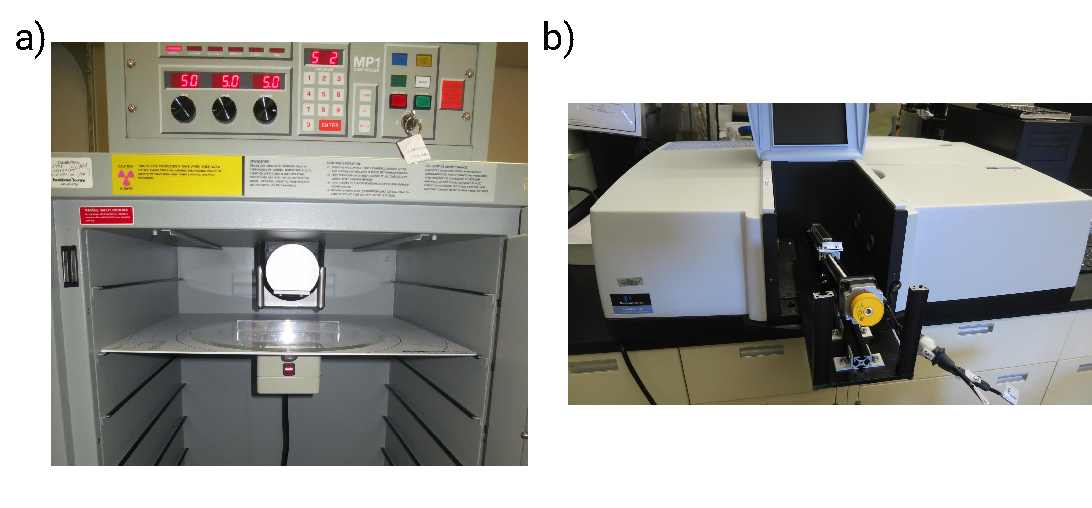
\includegraphics[width=\textwidth]{CUA_setup.pdf}
	\caption{X-ray source (a) and monochromator (b) used for testing the radiation hardness through transmission degradation of NLaK33 samples at Catholic University of America.}
	\label{fig:CUA_setup}
\end{figure}

%----------------------------------------------------------------------

%	HIGH-B TESTS SECTION
%----------------------------------------------------------------------

\section{Performance of MCP-PMTs in High Magnetic Field}
Due to the limiting space requirements of the EIC DIRC design, as mentioned in Chapter \ref{ch:eicdirc}, this places a unique set of requirements on the DIRC readout sensors. In order to achieve the desired single photon resolution while maintaining a sufficiently sized expansion volume the sensors, and therefore the pixels, must be small. Furthermore, due to the positioning of the readout plane being inside the large field of the solenoid magnet (see Figure \ref{fig:jleic_layout}) these sensors must also have a high tolerance to magnetic fields, both in magnitude (up to 3 T or higher), non-uniformity, and orientation. It was with these requirements in mind that the use of Micro-channel plate photomultiplier tubes (MCP-PMTs) was proposed (Figure \ref{fig:MCP_schematic}). MCP-PMTs have a much higher resistance to external magnetic fields than traditional photomultipliers, with studies being done up to 2 T \cite{MCPTest1}, \cite{MCPTest2}, \cite{MCPTest3}, \cite{MCPTest4}, \cite{MCPTest5}, \cite{MCPTest6}. The tests described below are the first to study the effects of fields as large as 5 T on MCP-PMTs.

\begin{figure}[ht]
	\centering
	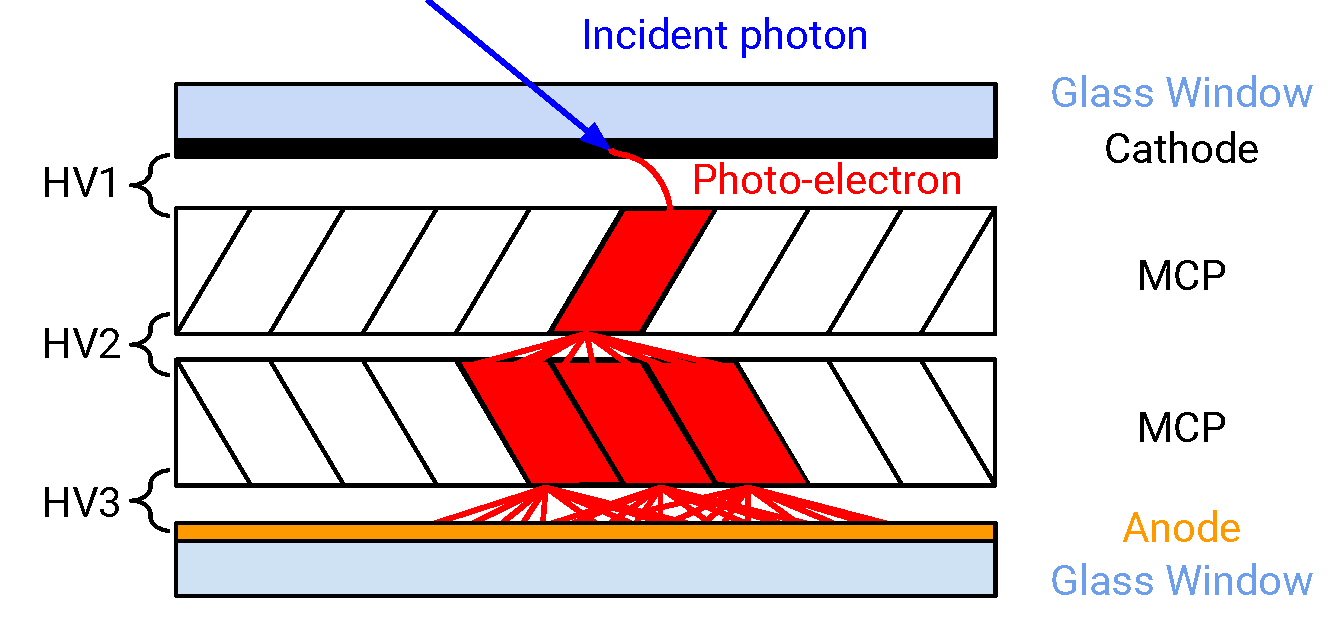
\includegraphics[width=\textwidth]{MCP_schematic.pdf}
	\caption{Schematic of the Micro-channel Plate photo-multiplier tube (MCP-PMT) concept. A cathode and anode sandwich two conducting plates with micrometer-sized channels (MCP) in a chevron pattern. An incident photon (blue) strikes the cathode, producing a photo-electron (red). That electron is accelerated through the potential difference between the cathode and first MCP (HV1) before striking the inside of one channel. This creates the same effect as an electron striking the dynode of a typical PMT, resulting in an avalanche of photo-electrons that emerge out of the other side of the first MCP. These electrons are again accelerated through a second potential difference (HV2) before repeating the process in the second MCP. Finally, the copious photo-electrons exit the second MCP, are accelerated through a final potential difference (HV3), and are collected on the anode. This design is both much more compact and much more resistant to magnetic fields compared to traditional PMTs.}
	\label{fig:MCP_schematic}
\end{figure}

In the fall of 2014 and summers of 2015 and 2016 several different MCP-PMTs were tested at Jefferson Lab \cite{HighB_DIRC2015}. The FROST  superconducting solenoidal magnet with a field tunable up to 5 T with a cylindrical bore diameter of 12.7 cm and a length of 76.2 cm was used for testing \cite{JLab_FrozenTarget}. The central field of the magnet, while quite large, is also very homogeneous, with an inhomogeneity of less than $5\times10^{-5}$ over a cylindrical volume with a diameter of 1.5 cm and a length of 5 cm. The sensors that were tested were held in place at the center of the magnet using a custom-built, non-magnetic, light-tight cylindrical dark box, as shown in Figure \ref{fig:highB_magnet}. Inside the dark box the sensor was held in place by a turn table that allowed for rotation around a vertical axis as well as a horizontal axis (the Y(Y') and Z(Z') axes in Figure \ref{fig:highB_schematics} respectively). The range of the polar angle $\theta$ was dependent on the size of the sensor being measured and the signal- and high-voltage cables connected to the back of the sensor. A cart allowed the sensor to move relative to the dark box for precise position and the center of the magnet.

A pulser-driven LED was used to illuminate the MCP-PMTs with 470 nm photons. An optical fiber was used to transmit the photons to the dark box and a diffuser installed inside the dark box cap was used to illuminate the entire face of the sensor with nearly constant intensity and 10 ns wide pulses at 30 kHz. The sensor signal output was then amplified using a 200-times preamplifier and used as input to a flash analog-to-digital converter (fADC). The fADC was then read out by our data acquisition system (DAQ).The pulser was also used as the trigger signal for the fADC, as shown in the chart in Figure \ref{fig:highB_schematics} (right).



\begin{figure}[ht]
	\centering
	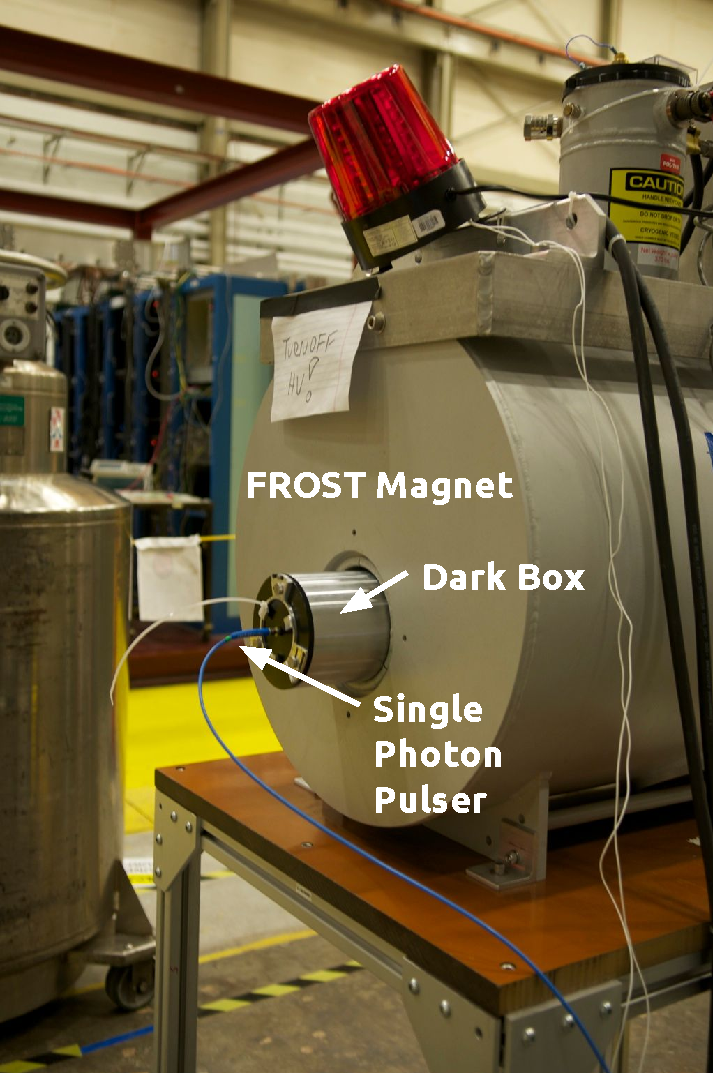
\includegraphics[width=0.4\textwidth]{highB_magnet.pdf}
	\caption{The FROST superconducting magnet with the dark box placed in the bore.}
	\label{fig:highB_magnet}
\end{figure}

\begin{figure}[ht]
	\centering
	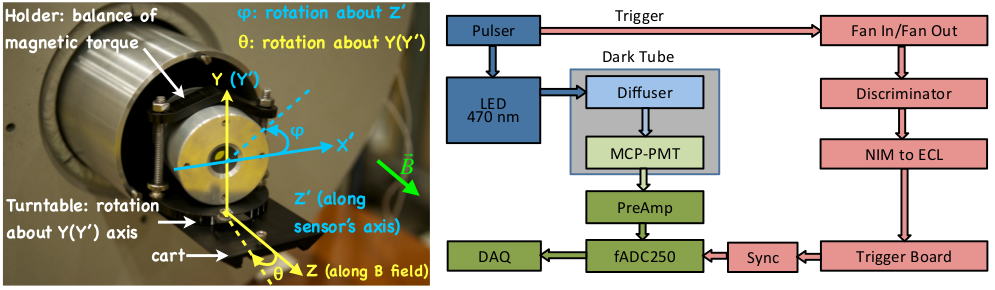
\includegraphics[width=\textwidth]{highB_schematics.png}
	\caption{Left: A closeup of the dark box showing the Photek PMT210 being held in place by the turn table. This setup allows the MCP-PMT to be rotated around both the horizontal Z(Z') axis as well as the vertical Y(Y') axis (with respect to the floor). The rotation about the Y(Y') and Z(Z') axes are described by the polar angle $\theta$ and azimuthal angle $\phi$ respectively. The magnetic field is parallel to the central axis of the dark box. Right: A flowchart of the readout used for testing. The photocathode is exposed to single 470 nm photons to produce photoelectrons, with a large voltage difference between the anode and cathode used to create an avalanche. The total charge is collected on the anode, amplified by a preamplifier, and digitized by an fADC and read out by a DAQ. \cite{HighB_DIRC2015} }
	\label{fig:highB_schematics}
\end{figure}